\section{Apprendimento Supervisionato}

\subsection{Modelli e metodologie utilizzate}

\paragraph{Modelli adottati.} Per qusto progetto ho deciso di adottare principalmente quattro modelli di apprendimento automatico:
\begin{itemize}[label=-]
    \item \textbf{Decision Tree}: classificatore strutturato ad albero in cui le foglie
    rappresentano le classi di appartenenza (o le probabilità di appartenenza a tali
    classi) mentre la radice e i nodi interni rappresentano delle condizioni sulle
    feature di input. A seconda se tali condizioni sono rispettate o meno, verrà
    seguito un percorso piuttosto che un altro e alla fine si arriverà alla classe di
    appartenenza
    \item \textbf{RandomForest}: classificatore che si ottiene creando tanti Decision Tree. Il valore in output si ottiene mediando sulle predizioni di ogni albero
    appartenente alla foresta (tecnica di bagging)
    \item \textbf{XGBoost} \cite{xgboost}: utilizza un approccio di boosting basato sul gradiente che combina diverse versioni di alberi decisionali deboli per creare un modello complessivo più potente
    \item \textbf{LightGBM} \cite{lightgbm}: altra libreria di boosting basata sul gradiente progettata per massimizzare l'efficienza computazionale. Si distingue per la sua velocità di addestramento e di previsione, grazie all'utilizzo di un algoritmo di divisione foglia-per-foglia e ad altre ottimizzazioni che minimizzano la memoria e la computazione necessarie.
\end{itemize}
\noindent Si è scelto di non usare modelli come ad esempio la regressione logistica, in quanto il rating può non essere direttamente correlato con le features a nostra disposizione (a titolo di esempio \cite{ilfattoquotidiano}), e quindi la linearità del modello non si presta bene. In alcuni esperimenti alcuni di questi modelli appena presentati sono stati sostituiti, in tal caso verrà specificato nella sezione apposita.
\paragraph{Train Test Split.} Per valutare le performance dei modelli, si è diviso il dataset in due parti: una parte per l'addestramento e una parte per la validazione. Si è scelto di adottare una divisione 80-20 \textbf{stratificata}, in modo da mantenere la stessa distribuzione delle classi nel training set e nel test set.
\paragraph{Cross-Validation.} Per trovare i migliori iperparametri per ogni modello e per la fase di valutazione si è adottata una \textit{Repeated Stratified K-fold cross validation}, in cui la cross validation viene ripetuta per $m$ volte mantenendo nei fold la distribuzione originaria delle classi. Il numero \textit{K} di fold è stato definito per ogni esperimento dalla regola di Sturges, una delle regole empiriche per la scelta del numero di classi in un istogramma. La regola di Sturges suggerisce di utilizzare un numero di classi (\textit{fold}) pari a $1 + \log_2(n)$, dove $n$ è il numero di osservazioni \textbf{del training set}. In questo caso, per garantire un numero di fold non troppo elevato mantenendo comunque la regola, si è scelto di adottare la regola usando la seguente formula: $\dfrac{1 + \log_2(n)}{3}$.
\paragraph{Ricerca degli iperparametri.} Per la ricerca degli iperparametri migliori si è adottata una \textit{GridSearchCV} con una \textit{Repeated Stratified K-fold Cross-Validation}. Di seguito la descrizione degli iperparametri per ogni modello e i valori testati:

\noindent\paragraph{Classificatore LightGBM.}
\begin{itemize}[leftmargin=*]
    \item \textbf{learning\_rate}: Velocità con cui il modello impara dai dati durante il processo di addestramento. Un learning rate più basso richiede più iterazioni per raggiungere la convergenza, ma può portare a una migliore generalizzazione e a modelli più stabili. D'altra parte, un learning rate più alto potrebbe accelerare il processo di addestramento. \textbf{Range di valori:} [0.01, 0.05, 0.1].
    \item \textbf{max\_depth}: Massima profondità dell'albero. \textbf{Range di valori:} [2, 5, 10].
    \item \textbf{n\_estimators}: Numero di alberi. \textbf{Range di valori:} [50, 100, 200].
    \item \textbf{lambda}: Parametro di regolarizzazione L2. Un valore più alto di lambda aumenta la forza della regolarizzazione, riducendo così il rischio di overfitting. \textbf{Range di valori:} [0.01, 0.1, 0.5].
    \item \textbf{num\_leaves}: Numero massimo di foglie per albero. \textbf{Range di valori:} [5, 15].
    \item \textbf{min\_gain\_to\_split}: Guadagno minimo richiesto per eseguire uno split. \textbf{Range di valori:} [0.1].
\end{itemize}

\noindent\paragraph{Classificatore DecisionTree.}
\begin{itemize}[leftmargin=*]
    \item \textbf{criterion}: Misura la qualità dello split effettuato sui nodi. \textbf{Range di valori:} ["gini", "entropy", "log\_loss"].\\
          \textit{Descrizioni:}
          \begin{itemize}
              \item \textbf{gini}: Misura la "purezza" della divisione dei dati, più precisamente quanto spesso un elemento viene classificato in modo sbagliato
              \item \textbf{entropy}: Misura la quantità di disordine nei dati. Minimizzare l'entropia significa massimizzare l'information gain
              \item \textbf{log\_loss}: Logarithmic loss, indicata quando l'output corrisponde a
              una probabilità piuttosto che a un valore di classe.
          \end{itemize}
    \item \textbf{max\_depth}: Massima profondità dell'albero. \textbf{Range di valori:} [5, 10, 20, 40].
    \item \textbf{min\_samples\_split}: Numero minimo di campioni per suddividere un nodo. \textbf{Range di valori:} [2, 5, 10, 20].
    \item \textbf{min\_samples\_leaf}: Numero minimo di campioni per essere foglia. \textbf{Range di valori:} [2, 5, 10, 20].
    \item \textbf{splitter}: Strategia di suddivisione del nodo. \textbf{Range di valori:} ["best"].
\end{itemize}

\noindent\paragraph{Classificatore RandomForest.}
\begin{itemize}[leftmargin=*]
    \item \textbf{criterion}: Criterio di suddivisione. \textbf{Range di valori:} ["gini", "entropy", "log\_loss"].\\
          \textit{Descrizioni:}
          \begin{itemize}
              \item \textbf{gini}: Misura la "purezza" della divisione dei dati, più precisamente quanto spesso un elemento viene classificato in modo sbagliato
              \item \textbf{entropy}: Misura la quantità di disordine nei dati. Minimizzare l'entropia significa massimizzare l'information gain
              \item \textbf{log\_loss}: Logarithmic loss, indicata quando l'output corrisponde a
              una probabilità piuttosto che a un valore di classe.
          \end{itemize}
    \item \textbf{n\_estimators}: Numero di alberi nella foresta. \textbf{Range di valori:} [10, 100, 200].
    \item \textbf{max\_depth}: Massima profondità dell'albero. \textbf{Range di valori:} [5, 10, 20].
    \item \textbf{min\_samples\_split}: Il numero minimo di esempi necessari affinché possa essere utilizzato un criterio di split. \textbf{Range di valori:} [2, 5, 10].
    \item \textbf{min\_samples\_leaf}: Il numero minimo di esempi per poter creare una foglia. \textbf{Range di valori:} [2, 5, 10].
\end{itemize}

\noindent\paragraph{Classificatore XGBoost.}
\begin{itemize}[leftmargin=*]
    \item \textbf{learning\_rate}: Velocità con cui il modello impara dai dati durante il processo di addestramento. Un learning rate più basso richiede più iterazioni per raggiungere la convergenza, ma può portare a una migliore generalizzazione e a modelli più stabili. D'altra parte, un learning rate più alto potrebbe accelerare il processo di addestramento. \textbf{Range di valori:} [0.01, 0.05, 0.10].
    \item \textbf{max\_depth}: Massima profondità degli alberi utilizzati. \textbf{Range di valori:} [5, 10, 20].
    \item \textbf{n\_estimators}: Numero di alberi utilizzati. \textbf{Range di valori:} [20, 50, 100].
    \item \textbf{lambda}: Parametro di regolarizzazione L2. Un valore più alto di lambda aumenta la forza della regolarizzazione, riducendo così il rischio di overfitting. \textbf{Range di valori:} [0.01, 0.1, 0.5].
\end{itemize}

\paragraph{Riproducibilità.} Per garantire la riproducibilità dei risultati, si è scelto di fissare il \textit{seed} per la generazione di numeri casuali al numero \textit{42}.
\paragraph{Valutazione.} La parte di valutazione è stata fatta utilizzando una \textit{cross\_val\_score}, ovvero un metodo che valuta sempre utilizzando la Cross Validation i modelli addestrati. Per la valutazione delle performance del sistema ho deciso di utilizzare le seguenti metriche:
\begin{itemize}[label=-]
    \item \textbf{Balanced Accuracy}: È una versione modificata dell'accuratezza standard che tiene conto dello sbilanciamento delle classi nei dati. Calcola la media delle accuratezze per ciascuna classe, fornendo quindi una valutazione equilibrata delle prestazioni del modello su tutte le classi. Utilizzare un'accuracy normale sarebbe fuorviante, al classificatore potrebbe bastare predire sempre la classe più frequente per ottenere un'accuracy alta, ma questo non significa che il classificatore sia buono. La balanced accuracy è definita come la media delle sensibilità per ciascuna classe.
    \item \textbf{Cohen's Kappa} \cite{kappa}: è una misura della concordanza tra le predizioni di un classificatore e i veri valori delle classi, correggendo l'accordo che potrebbe verificarsi solo per caso. Questa metrica tiene conto dell'equilibrio tra le classi e fornisce una valutazione più accurata rispetto alla semplice accuratezza. Il valore di Cohen's Kappa varia da -1 a 1, dove 1 indica una perfetta concordanza tra le predizioni e i veri valori, 0 indica concordanza casuale e valori negativi indicano concordanza peggiore di quella casuale
    \item \textbf{Geometric Mean}: è la radice del prodotto della sensibilità per classe. Questa misura cerca di massimizzare l'accuratezza su ciascuna delle classi, mantenendo queste accuratezze bilanciate. Per i problemi multiclasse è la radice n-esima del prodotto della sensibilità per ciascuna classe. Se almeno una classe non viene riconosciuta dal classificatore, la geometric mean sarà 0, pertanto ci servirà per dare soprattutto un \textit{lower bound} di confronto per i nostri modelli.
\end{itemize}
\noindent La \textit{GridSearchCV} è stata allenata nel trovare gli iperparametri che massimizzano la \textit{Balanced accuracy}. Sono state poi prese in considerazione \textbf{varianza} e \textbf{deviazione standard} per ogni modello: un modello con una varianza e una deviazione standard più basse è preferibile, in quanto indica che le predizioni sono più coerenti e affidabili.

\subsection{Primo esperimento}
\noindent Nel primo esperimento si è provato ad allenare i modelli proposti in precedenza sugli esempi del dataset senza alcuna manipolazione successiva a quelle raccontate in precedenza. Sono state utilizzate le metriche e i modelli proposti in precedenza.

\paragraph{Iperparametri.} Di seguito si riportano gli iperparametri ottenuti dalla \textit{GridSearchCV} per ogni modello:
    
        
        \begin{table}[H]
            \centering
            \begin{tabular}{|l|l|}
            \hline
            \textbf{Parametro}                 & \textbf{Valore} \\ \hline
            LightGBM\_\_learning\_rate            & 0.1             \\ \hline
            LightGBM\_\_max\_depth                & 10              \\ \hline
            LightGBM\_\_n\_estimators             & 200             \\ \hline
            LightGBM\_\_lambda                    & 0.1             \\ \hline
            LightGBM\_\_num\_leaves               & 15              \\ \hline
            LightGBM\_\_min\_gain\_to\_split      & 0.1             \\ \hline
            LightGBM\_\_verbose                   & 0               \\ \hline
            XGBoost\_\_learning\_rate         & 0.1             \\ \hline
            XGBoost\_\_max\_depth             & 10              \\ \hline
            XGBoost\_\_n\_estimators          & 100             \\ \hline
            XGBoost\_\_lambda                 & 0.1             \\ \hline
            DecisionTree\_\_criterion         & log\_loss       \\ \hline
            DecisionTree\_\_max\_depth        & 40              \\ \hline
            DecisionTree\_\_min\_samples\_split & 5               \\ \hline
            DecisionTree\_\_min\_samples\_leaf & 2               \\ \hline
            RandomForest\_\_n\_estimators     & 100             \\ \hline
            RandomForest\_\_max\_depth        & 20              \\ \hline
            RandomForest\_\_min\_samples\_split & 2               \\ \hline
            RandomForest\_\_min\_samples\_leaf & 2               \\ \hline
            RandomForest\_\_criterion         & log\_loss       \\ \hline
            \end{tabular}
            \caption{Parametri del modello}
            
            \end{table}
\paragraph{Risultati.} Di seguito si riportano i risultati ottenuti per ogni metrica e per ogni modello:
\begin{figure}[H]
    \centering
    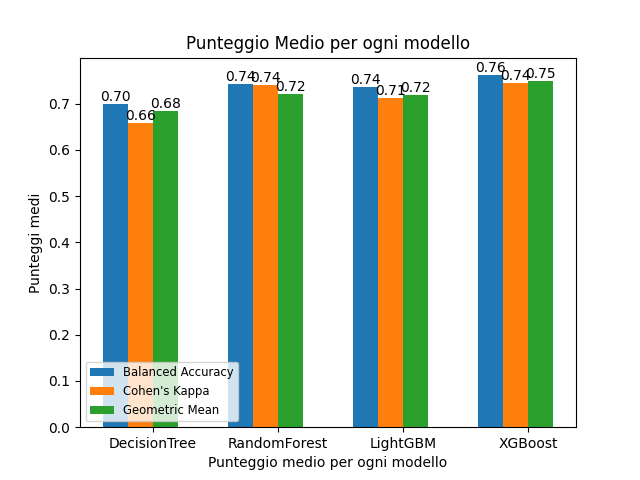
\includegraphics[scale=0.5]{img/normal_metrics.png}
\end{figure}


\paragraph{Curve di apprendimento.} Di seguito si riportano le curve di apprendimento per ogni modello, con tanto di deviazione standard e varianza:

\begin{figure}[H]
    \centering
    \begin{minipage}[b]{0.45\linewidth}
      \centering
      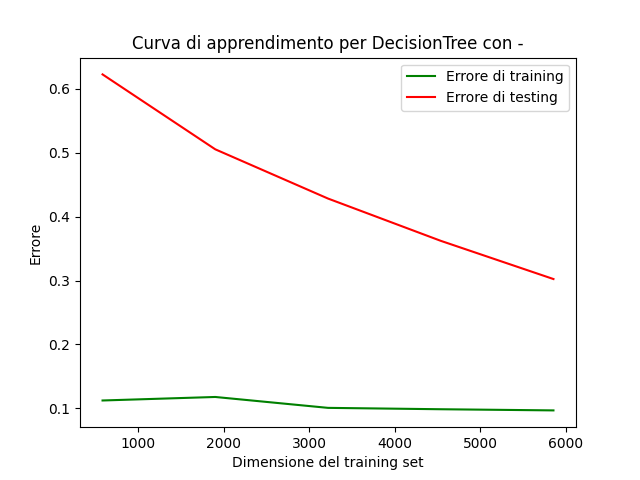
\includegraphics[scale=0.5]{img/learning_curve_DecisionTree_-.png}
      
    \end{minipage}
    \hfill
    \begin{minipage}[b]{0.45\linewidth}
      \centering
      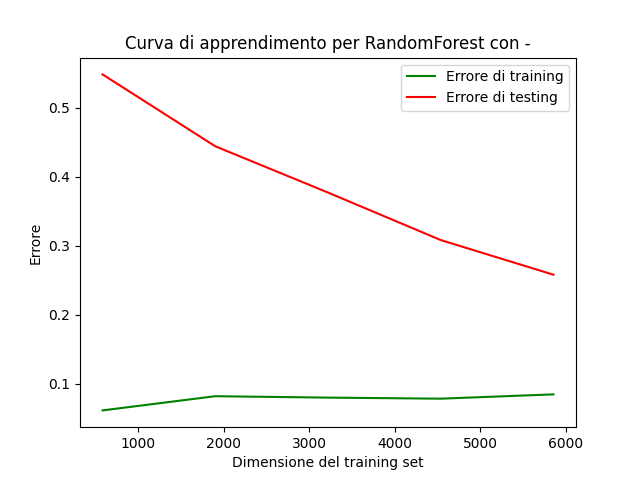
\includegraphics[scale=0.5]{img/learning_curve_RandomForest_-.png}
      
    \end{minipage}
    
    \begin{minipage}[b]{0.45\linewidth}
      \centering
      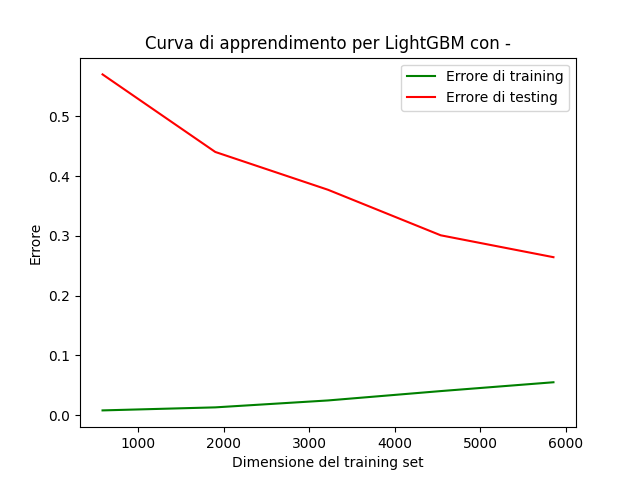
\includegraphics[scale=0.5]{img/learning_curve_LightGBM_-.png}
      
    \end{minipage}
    \hfill
    \begin{minipage}[b]{0.45\linewidth}
      \centering
      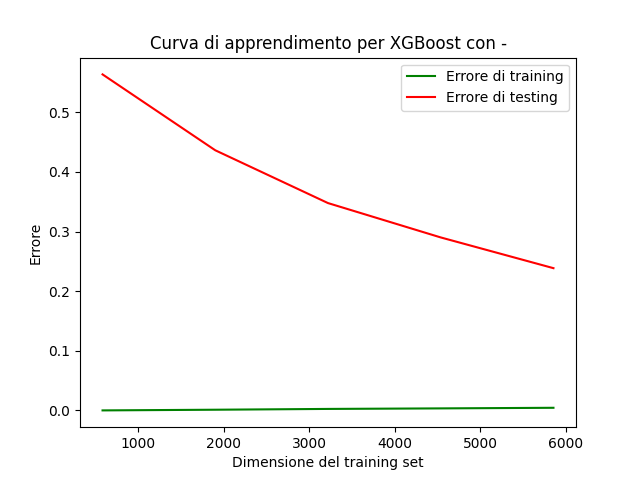
\includegraphics[scale=0.5]{img/learning_curve_XGBoost_-.png}
      
    \end{minipage}
    \caption{Curve di apprendimento.}
    
    \end{figure}

\begin{table}[H]
    \centering
    \begin{tabular}{lcc}
    \toprule
    \textbf{Modello} & \textbf{Train Error Std} & \textbf{Test Error Std} \\
    \midrule
    LightGBM & 0.003677832760964418 & 0.014729799395024678 \\
    XGBoost & 0.0017806001233474666 & 0.014258802458827638 \\
    DecisionTree & 0.004798633588628468 & 0.015296962637326389 \\
    RandomForest & 0.004364244206597904 & 0.014128073154668751 \\
    \bottomrule
    \end{tabular}
    \caption{Deviazione standard dell'errore per i Modelli}
    
\end{table}

\begin{table}[H]
    \centering
    \begin{tabular}{lcc}
    \toprule
    \textbf{Modello} & \textbf{Train Error Var} & \textbf{Test Error Var} \\
    \midrule
    LightGBM & 1.3526453817623153e-05 & 0.00021696699021766939 \\
    XGBoost & 3.1705367992650135e-06 & 0.00020331344755986913 \\
    DecisionTree & 2.3026884317913326e-05 & 0.0002339970659277595 \\
    RandomForest & 1.9046627494823375e-05 & 0.00019960245106367185 \\
    \bottomrule
    \end{tabular}
    \caption{Varianza degli Errori per i Modelli}
    
\end{table}

\paragraph{Feature importance.} E' stata raccolta anche l'informazione riguardo quali feature abbiano contribuito di più in ogni modello per le predizioni.
\\Questo è stato fatto nel primo esperimento, in modo da utilizzare le feature maggiormente predittive per i modelli considerati migliori per costruire la rete bayesiana. Si riporta di seguito solo il grafico relativo al Random Forest, per non appesantire la trattazione, gli altri sono disponibili nel repository:

\begin{figure}[H]
    \centering
    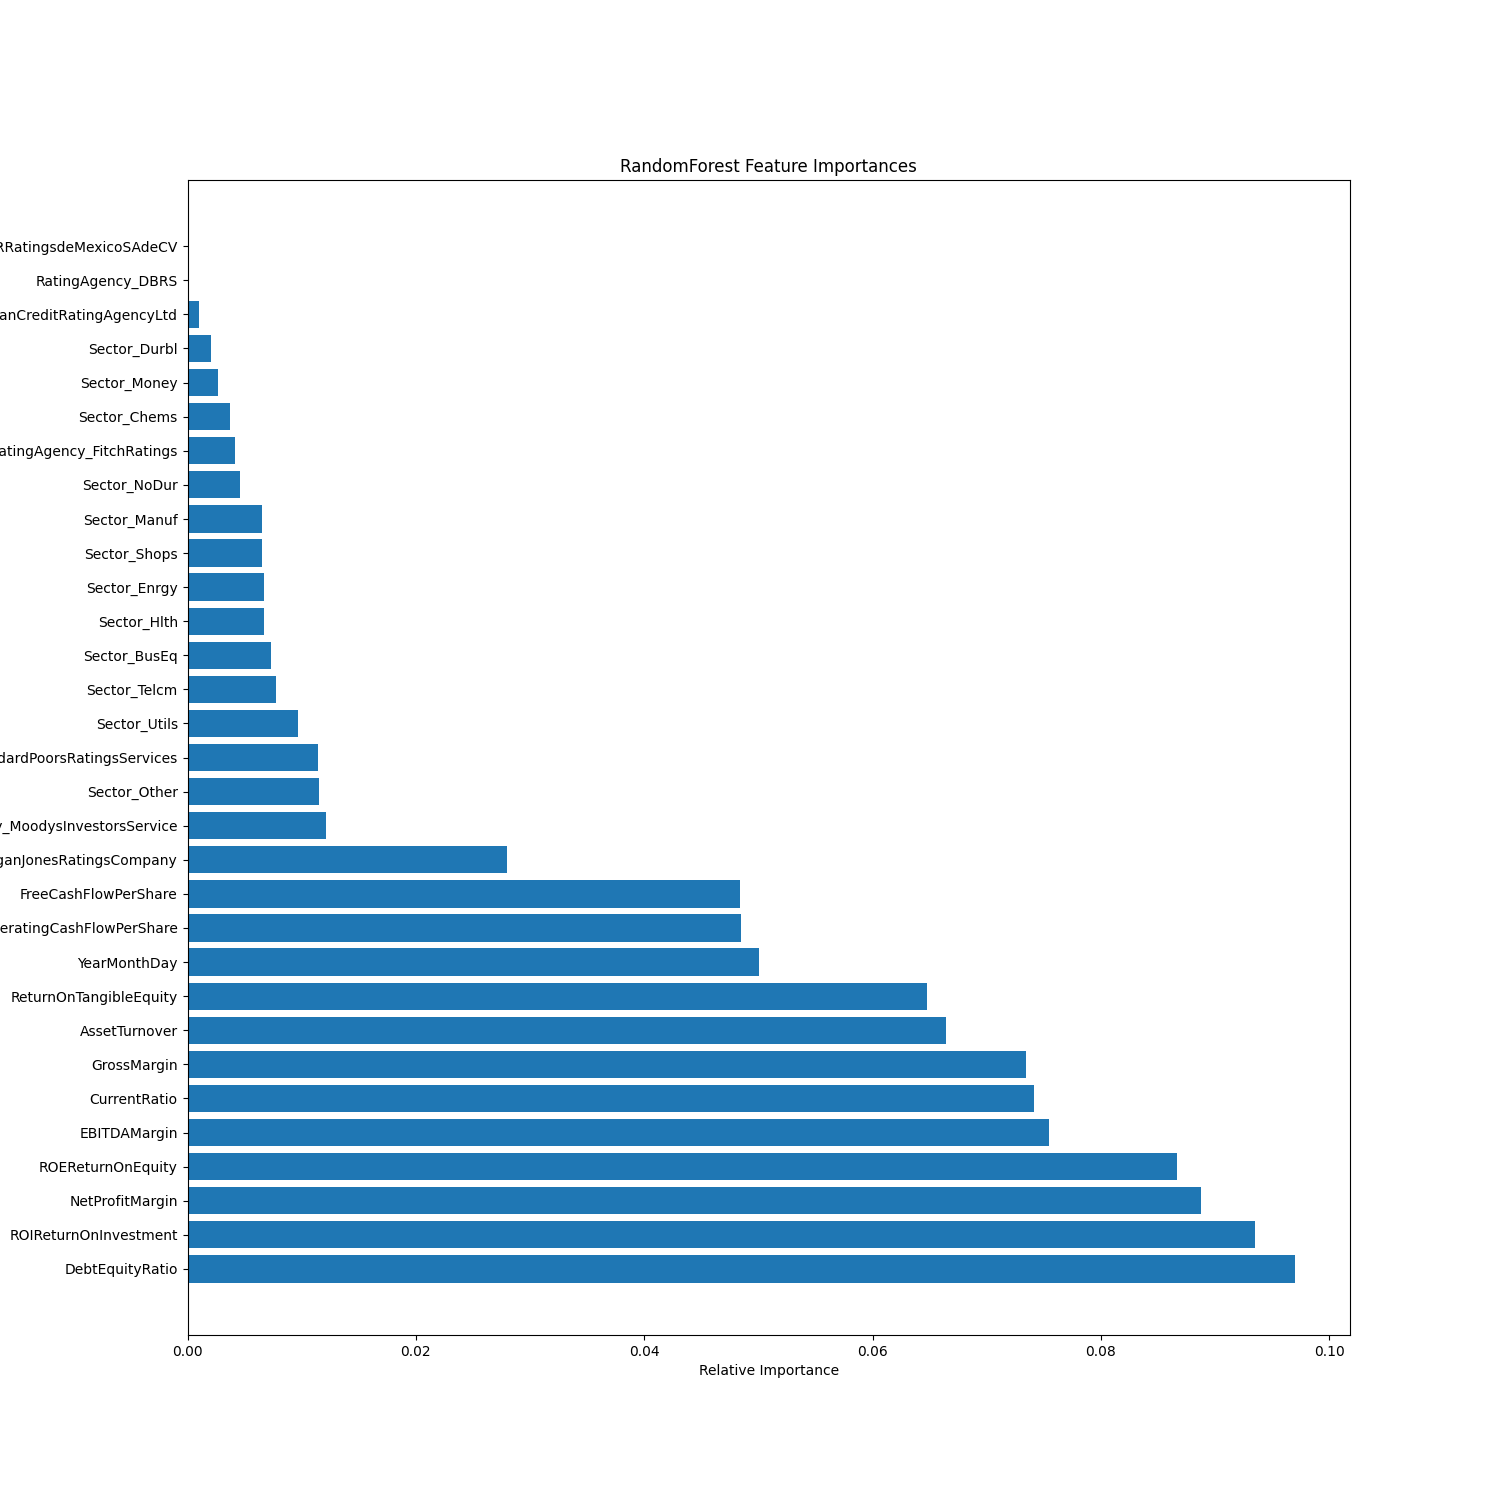
\includegraphics[scale=0.35]{img/feature_importances_RandomForest.png}
\end{figure}

\paragraph{Valutazione.} I primi risultati sono incoraggianti, soprattutto per i modelli basati su boosting e bagging, un pò meno per il decision tree. Le metriche non ci danno informazioni particolarmente utili riguardante un possibile overfitting o underfitting, però ci fanno capire come già di base i modelli si comportano abbastanza bene. \\
Il \textbf{Decision Tree} non sembra dare segni di overfitting quanto quasi più di underfitting, dato che l'errore di training si stabilizza dopo circa metà training set, ma l'errore di testing è ancora in discesa ed è un pò lontano dall'errore di traning. Il \textbf{Random Forest} presenta un piccolo picco nell'errore di training dopo circa 2000 esempi, stessa cosa dopo altri 2000, ma comunque sono picchi poco significativi, anche qui l'errore di testing è abbastanza lontano, quindi non si può parlare di overfitting. Il \textbf{LightGBM} mostra dei possibili primi segnali di overfitting: l'errore di training inizia ad aumentare col tempo, l'errore di testing inizia a scendere abbastanza velocemente. L'\textbf{XGBoost} non presenta problemi, riesce ad essere allenato senza problemi, ma l'errore di testing è comunque ancora abbastanza alto, quindi non si può parlare di overfitting. In conclusione, i modelli non presentano segni di overfitting, ma il LightGBM potrebbe presentare dei segni di overfitting in futuro.



\subsection{Secondo esperimento: class weights vs BalancedRF}
\noindent La tecnica del class weight assegna pesi differenti alle classi durante il processo di addestramento del modello. In particolare, si attribuiscono pesi maggiori alle classi minoritarie e pesi minori alle classi maggioritarie. Questo consente al modello di dare maggiore importanza alle istanze delle classi minoritarie durante l'addestramento. In questo modo, il modello sarà in grado di apprendere meglio le caratteristiche delle classi minoritarie e di migliorare le prestazioni su queste classi.\\
I pesi delle classi possono essere calcolati in diversi modi. Uno dei metodi comuni è utilizzare l'inverso della frequenza delle classi nel dataset, che è la tecnica che andremo ad utilizzare.\\ \\ Per questo esperimento, andremo a usare tre modelli, tagliando fuori l'XGBoost, in quanto non supporta nativamente la possibilità di assegnare un peso alle classi.\\ In alternativa si utilizzerà un \textit{BalancedRandomForest}, che si differenzia dal classico \textit{Random Forest} per il fatto che estrarrà un campione su cui allenare ogni singolo \textit{decision tree} dalla classe di minoranza e campionerà con sostituzione lo stesso numero di campioni dalla classe di maggioranza. E' un modello che si presta bene proprio per classificazione con classi sbilanciate, pertanto lo testeremo contro dei modelli impostati con un \textbf{bias} verso le classi minoritarie.

\paragraph{Iperparametri.} Per il BalancedRandomForest lo spazio di ricerca degli iperparametri scelto è il medesimo dei Random Forest. Di seguito si riportano gli iperparametri ottenuti dalla \textit{GridSearchCV} per ogni modello:

\begin{table}[H]
\centering
\begin{tabular}{|l|l|}
\toprule
\textbf{Parametro}                 & \textbf{Valore} \\ \midrule
BalancedRandomForest\_\_criterion & entropy \\ 
BalancedRandomForest\_\_n\_estimators & 200 \\
BalancedRandomForest\_\_max\_depth & 20 \\
BalancedRandomForest\_\_min\_samples\_split & 2 \\
BalancedRandomForest\_\_min\_samples\_leaf & 2 \\
BalancedRandomForest\_\_sampling\_strategy & all \\
BalancedRandomForest\_\_replacement & True \\
LightGBM\_\_learning\_rate & 0.1 \\
LightGBM\_\_max\_depth & 10 \\
LightGBM\_\_n\_estimators & 200 \\
LightGBM\_\_lambda & 0.5 \\
LightGBM\_\_num\_leaves & 15 \\
LightGBM\_\_min\_gain\_to\_split & 0.1 \\
LightGBM\_\_verbose & 0 \\
LightGBM\_\_class\_weight & balanced \\
DecisionTree\_\_criterion & entropy \\
DecisionTree\_\_max\_depth & 40 \\
DecisionTree\_\_min\_samples\_split & 2 \\
DecisionTree\_\_min\_samples\_leaf & 2 \\
DecisionTree\_\_class\_weight & balanced \\
RandomForest\_\_n\_estimators & 200 \\
RandomForest\_\_max\_depth & 20 \\
RandomForest\_\_min\_samples\_split & 10 \\
RandomForest\_\_min\_samples\_leaf & 2 \\
RandomForest\_\_criterion & log\_loss \\
RandomForest\_\_class\_weight & balanced \\ \bottomrule
\end{tabular}
\caption{Parametri del modello}
\end{table}

\paragraph{Risultati.} Di seguito si riportano i risultati ottenuti per ogni metrica e per ogni modello:

\begin{figure}[H]
    \centering
    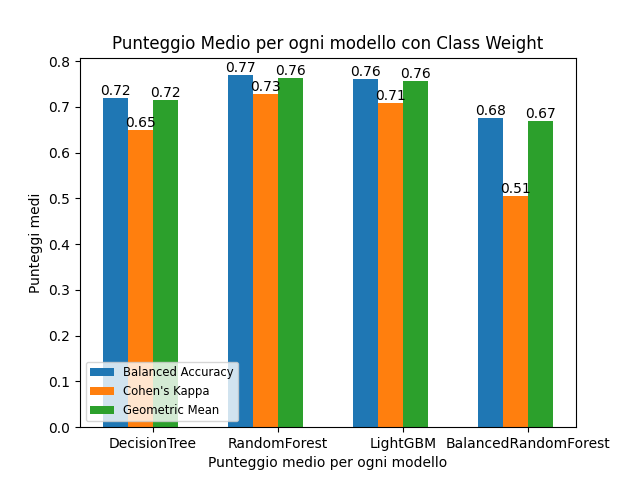
\includegraphics[scale=0.7]{img/cw_metrics.png}
\end{figure}



\paragraph{Curve di apprendimento.} Di seguito si riportano le curve di apprendimento per ogni modello, con tanto di deviazione standard e varianza:

\begin{figure}[H]
    \centering
    \begin{minipage}[b]{0.45\linewidth}
      \centering
      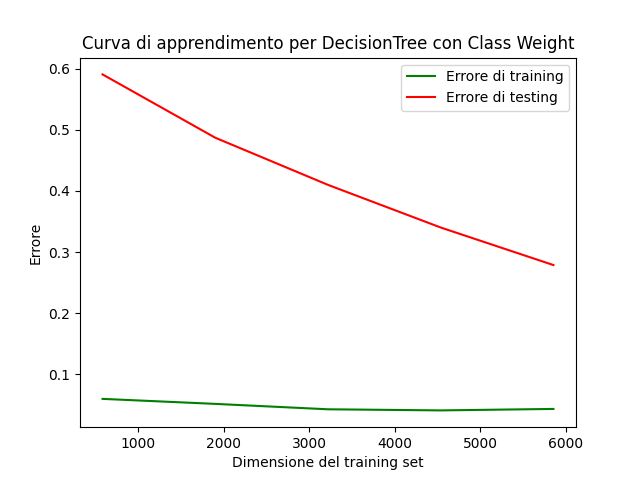
\includegraphics[scale=0.5]{img/learning_curve_DecisionTree_Class Weight.png}
      
    \end{minipage}
    \hfill
    \begin{minipage}[b]{0.45\linewidth}
      \centering
      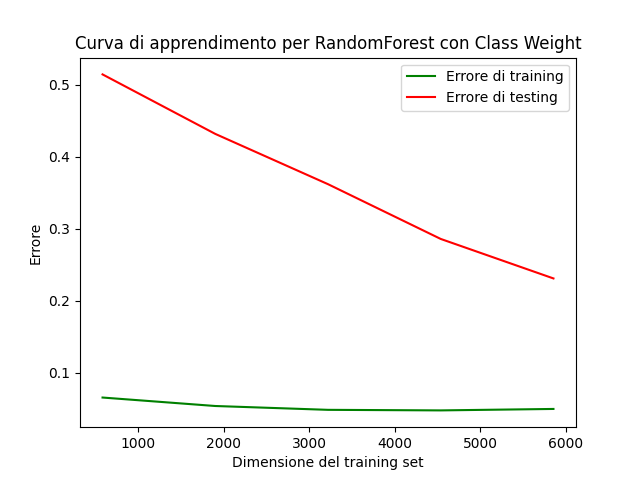
\includegraphics[scale=0.5]{img/learning_curve_RandomForest_Class Weight.png}
      
    \end{minipage}
    
    \begin{minipage}[b]{0.45\linewidth}
      \centering
      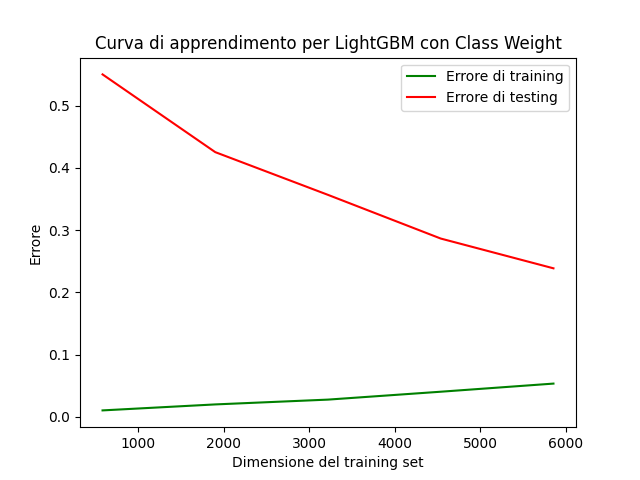
\includegraphics[scale=0.5]{img/learning_curve_LightGBM_Class Weight.png}
      
    \end{minipage}
    \hfill
    \begin{minipage}[b]{0.45\linewidth}
      \centering
      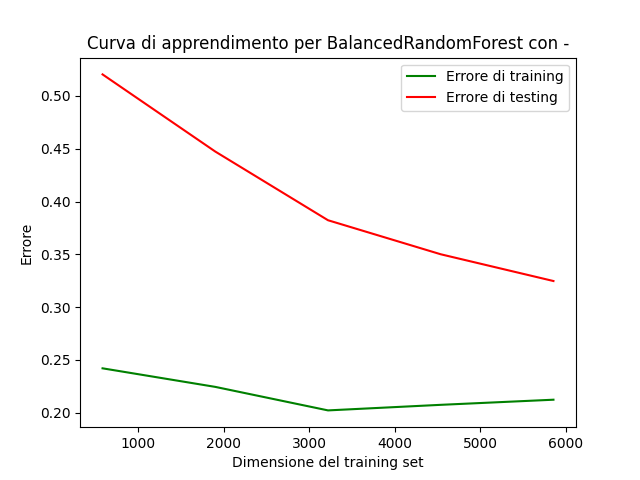
\includegraphics[scale=0.5]{img/learning_curve_BalancedRandomForest_-.png}
      
    \end{minipage}
    \caption{Curve di apprendimento.}
    
    \end{figure}

\begin{table}[H]
    \centering
    \begin{tabular}{lcc}
    \toprule
    \textbf{Modello} & \textbf{Train Error Std} & \textbf{Test Error Std} \\
    \midrule
    LightGBM & 0.0026561375826418482 & 0.016525860583798364 \\
    BalancedRandomForest & 0.004339002154983959 & 0.009953134681109565\\
    DecisionTree & 0.0015879855371825314 & 0.015329002342180082 \\
    RandomForest & 0.0018445912002196091 & 0.02129919916812779 \\
    \bottomrule
    \end{tabular}
    \caption{Deviazione standard dell'errore per i Modelli}
\end{table}


\begin{table}[H]
    \centering
    \begin{tabular}{lcc}
    \toprule
    \textbf{Modello} & \textbf{Train Error Var} & \textbf{Test Error Var} \\
    \midrule
    LightGBM & 7.055066857922481e-06 & 0.0002731040680351404 \\
    BalancedRandomForest & 1.8826939700955435e-05 & 9.906488998030602e-05 \\
    DecisionTree & 2.5216980663008927e-06 & 0.00023497831280656247 \\
    RandomForest & 3.4025166959276185e-06 & 0.00045365588520357555 \\
    \bottomrule
    \end{tabular}
    \caption{Varianza degli Errori per i Modelli}
\end{table}

\paragraph{Valutazione.} A un primo impatto possiamo vedere come il BalancedRandomForest non è riuscito a mantenere le aspettative, soprattutto se confrontato con il suo "gemello", il Random Forest classico. \\ Rispetto al primo esperimento, le metriche di tutti gli altri modelli sono leggermente migliorate, ma siamo molto vicini ai range di varianza e deviazione standard del primo esperimento. Il Decision Tree sembra essersi stabilizzato ancora di più, il Random Forest presenta un errore di training decisamente più lineare, il LightGBM non presenta miglioramenti.

\subsection{Terzo esperimento: oversampling}
\noindent L'oversampling consiste nell'aumentare artificialmente il numero di esempi delle classi minoritarie nel dataset di addestramento, in modo da bilanciare meglio la distribuzione delle classi. Ciò viene fatto replicando casualmente le istanze esistenti della classe minoritaria o generando nuove istanze sintetiche utilizzando tecniche come lo SMOTE, che testeremo. \\SMOTE sintetizza nuove istanze per la classe minoritaria creando campioni artificiali lungo le linee che collegano istanze simili nello spazio delle feature. In questo modo, si cerca di mantenere la struttura dei dati originari mentre si aumenta il numero di istanze della classe minoritaria. \\ Andremo a confrontare lo SMOTE con i risultati degli altri esperimenti e con quelli dell'ADASYN, un'altra tecnica di oversampling.\\ ADASYN genera nuovi esempi per le istanze delle classi minoritarie che hanno un alto grado di disomogeneità, ovvero che sono il più possibile differenti dagli esempi della classe maggioritaria per caratteristiche. Questa tecnica a differenza della precedente non riesce a garantire il perfetto ribilanciamento del dataset, ma ad ogni modo riesce quasi del tutto a risanarlo tranne nei casi in cui gli esempi della classe minoritaria sono sparsi e immersi in esempi di classe maggioritaria. \\ Gli algoritmi sono stati utilizzati con 
\textit{random\_state} uguale a \textit{42}, e con \textit{sampling\_strategy} uguale a \textit{all}, in modo da ribilanciare tutte le classi. Come sviluppo futuro si potrebbe pensare di fare una sorta di \textit{GridSearchCV} per trovare il miglior set di parametri per queste tecniche.
\begin{attenzione}
Si è prestata particolare attenzione nell'applicazione delle tecniche descritte nel seguito del capitolo. Infatti un errore comune è quello di utilizzare tecniche di oversampling, undersampling o miste su tutto il dataset, andando quindi ad allenare il modello sui dati sintetici, ma anche ad usare un test set con dati sintetici, che non rispecchia la realtà. Per questo motivo, si applicano le tecniche di oversampling soltanto sul training set, e non sul test set. Questo potrebbe portare a miglioramenti che non risultano entusiasmanti, ma è comunque la scelta migliore per valutare i nostri modelli.
\end{attenzione}

\subsubsection{SMOTE}
\paragraph{Iperparametri.} Di seguito si riportano gli iperparametri ottenuti dalla \textit{GridSearchCV} per ogni modello:

\begin{table}[H]
    \centering
    \begin{tabular}{|l|l|}
    \toprule
    \textbf{Parametro}                 & \textbf{Valore} \\ \midrule
    LightGBM\_\_learning\_rate            & 0.1             \\ 
    LightGBM\_\_max\_depth                & 10              \\ 
    LightGBM\_\_n\_estimators             & 200             \\ 
    LightGBM\_\_lambda                    & 0.01            \\ 
    LightGBM\_\_num\_leaves               & 15              \\ 
    LightGBM\_\_min\_gain\_to\_split      & 0.1             \\ 
    XGBoost\_\_learning\_rate         & 0.1             \\ 
    XGBoost\_\_max\_depth             & 10              \\ 
    XGBoost\_\_n\_estimators          & 100             \\ 
    XGBoost\_\_lambda                 & 0.01            \\ 
    DecisionTree\_\_criterion         & gini            \\ 
    DecisionTree\_\_max\_depth        & 20              \\ 
    DecisionTree\_\_min\_samples\_split & 5               \\ 
    DecisionTree\_\_min\_samples\_leaf & 2               \\ 
    RandomForest\_\_n\_estimators     & 200             \\ 
    RandomForest\_\_max\_depth        & 20              \\ 
    RandomForest\_\_min\_samples\_split & 2               \\ 
    RandomForest\_\_min\_samples\_leaf & 2               \\ 
    RandomForest\_\_criterion         & entropy         \\ \bottomrule
    \end{tabular}
    \caption{Parametri del modello}
    \end{table}

\paragraph{Risultati.} Di seguito si riportano i risultati ottenuti per ogni metrica e per ogni modello:

\begin{figure}[H]
    \centering
    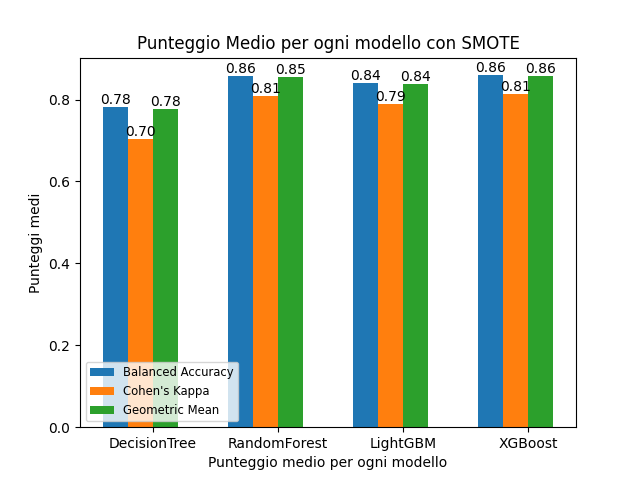
\includegraphics[scale=0.7]{img/smote_metrics.png}
\end{figure}



\paragraph{Curve di apprendimento.} Di seguito si riportano le curve di apprendimento per ogni modello, con tanto di deviazione standard e varianza:

\begin{figure}[H]
    \centering
    \begin{minipage}[b]{0.45\linewidth}
      \centering
      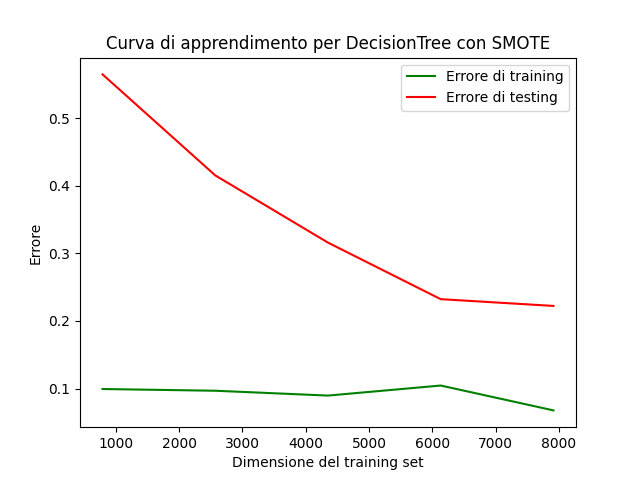
\includegraphics[scale=0.5]{img/learning_curve_DecisionTree_SMOTE.png}
      
    \end{minipage}
    \hfill
    \begin{minipage}[b]{0.45\linewidth}
      \centering
      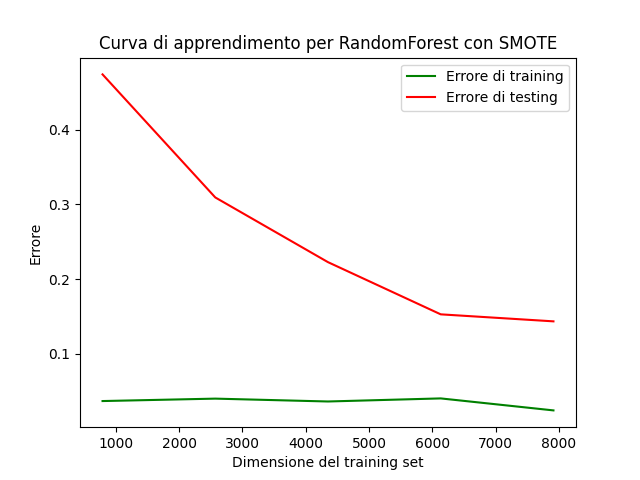
\includegraphics[scale=0.5]{img/learning_curve_RandomForest_SMOTE.png}
      
    \end{minipage}
    
    \begin{minipage}[b]{0.45\linewidth}
      \centering
      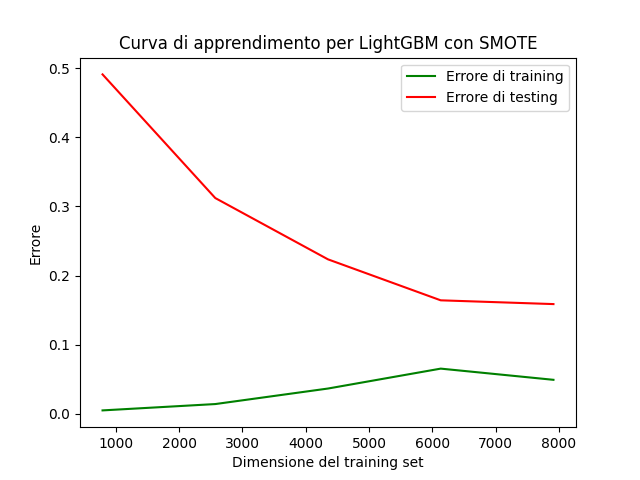
\includegraphics[scale=0.5]{img/learning_curve_LightGBM_SMOTE.png}
      
    \end{minipage}
    \hfill
    \begin{minipage}[b]{0.45\linewidth}
      \centering
      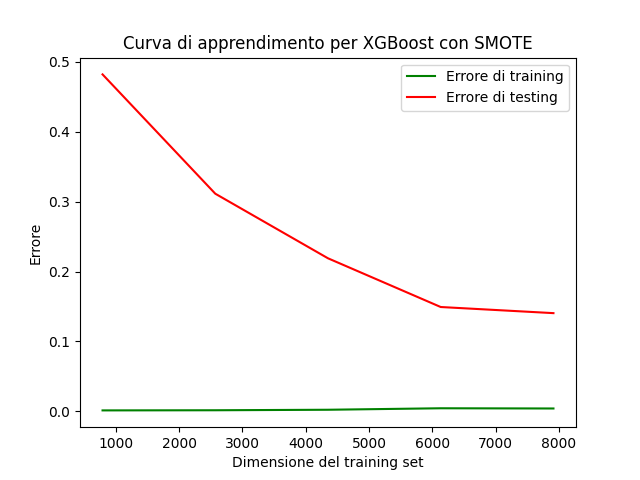
\includegraphics[scale=0.5]{img/learning_curve_XGBoost_SMOTE.png}
      
    \end{minipage}
    \caption{Curve di apprendimento.}
    
    \end{figure}

\begin{table}[H]
    \centering
    \begin{tabular}{lcc}
    \toprule
    \textbf{Modello} & \textbf{Train Error Std} & \textbf{Test Error Std} \\
    \midrule
    LightGBM & 0.0013274976900467363 & 0.005557462071090911 \\
    XGBoost & 0.0010996943494845943 & 0.007626860052066837 \\
    DecisionTree & 0.005071533109955392 & 0.006148834960506031 \\
    RandomForest & 0.000739498264938402 & 0.004926394385656445 \\
    \bottomrule
    \end{tabular}
    \caption{Deviazione standard dell'errore per i Modelli}
\end{table}

\begin{table}[H]
    \centering
    \begin{tabular}{lcc}
    \toprule
    \textbf{Modello} & \textbf{Train Error Var} & \textbf{Test Error Var} \\
    \midrule
    LightGBM & 1.7622501170794206e-06 & 3.088538467161408e-05 \\
    XGBoost & 1.209327662288345e-06 & 5.816899425381296e-05 \\
    DecisionTree & 2.5720448085373803e-05 & 3.7808171371541206e-05 \\
    RandomForest & 5.468576838469069e-07 & 2.426936164302734e-05 \\
    \bottomrule
    \end{tabular}
    \caption{Varianza degli Errori per i Modelli}
\end{table}

\paragraph{Valutazione.} I risultati sono decisamente migliori rispetto ai due esperimenti precedenti, pertanto resta da controllare se vi è overfitting in qualche modello. \\ I valori di deviazione standard e varianza non portano a pensare a overfitting. Guardando le curve notiamo come l'XGBoost si sia comportato bene, stessa cosa per il Random Forest, mentre sorgono dubbi sull'efficacia del Decision Tree e del LightGBM, in particolare quest'ultimo sembra raggiungere una configurazione ideale tra i 6000 e gli 8000 esempi.

\subsubsection{ADASYN}
\paragraph{Iperparametri.} Di seguito si riportano gli iperparametri ottenuti dalla \textit{GridSearchCV} per ogni modello:

\begin{table}[H]
    \centering
    \begin{tabular}{|l|l|}
    \toprule
    \textbf{Parametro}                 & \textbf{Valore} \\ \midrule
    LightGBM\_\_learning\_rate            & 0.1             \\ 
    LightGBM\_\_max\_depth                & 10              \\ 
    LightGBM\_\_n\_estimators             & 200             \\ 
    LightGBM\_\_lambda                    & 0.1             \\ 
    LightGBM\_\_num\_leaves               & 15              \\ 
    LightGBM\_\_min\_gain\_to\_split      & 0.1             \\ 
    XGBoost\_\_learning\_rate         & 0.1             \\ 
    XGBoost\_\_max\_depth             & 20              \\ 
    XGBoost\_\_n\_estimators          & 100             \\ 
    XGBoost\_\_lambda                 & 0.01            \\ 
    DecisionTree\_\_criterion         & gini            \\ 
    DecisionTree\_\_max\_depth        & 40              \\ 
    DecisionTree\_\_min\_samples\_split & 5               \\ 
    DecisionTree\_\_min\_samples\_leaf & 2               \\ 
    RandomForest\_\_n\_estimators     & 200             \\ 
    RandomForest\_\_max\_depth        & 20              \\ 
    RandomForest\_\_min\_samples\_split & 2               \\ 
    RandomForest\_\_min\_samples\_leaf & 2               \\ 
    RandomForest\_\_criterion         & log\_loss         \\ \bottomrule
    \end{tabular}
    \caption{Parametri del modello}
    \end{table}

\paragraph{Risultati.} Di seguito si riportano i risultati ottenuti per ogni metrica e per ogni modello:

\begin{figure}[H]
    \centering
    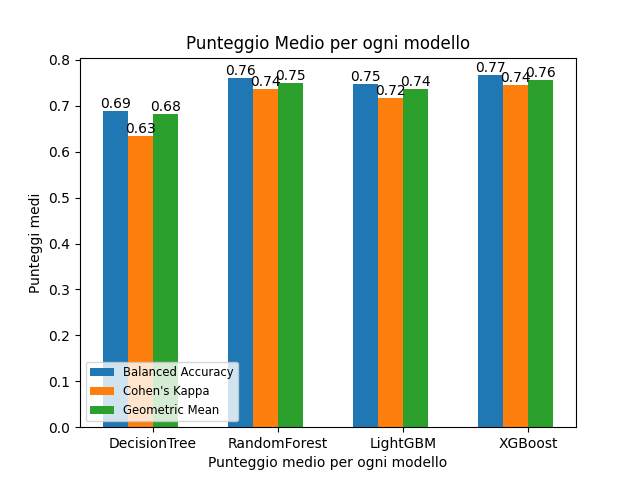
\includegraphics[scale=0.7]{img/adasyn_metrics.png}
\end{figure}

\paragraph{Curve di apprendimento.} Di seguito si riportano le curve di apprendimento per ogni modello, con tanto di deviazione standard e varianza:

\begin{figure}[H]
    \centering
    \begin{minipage}[b]{0.45\linewidth}
      \centering
      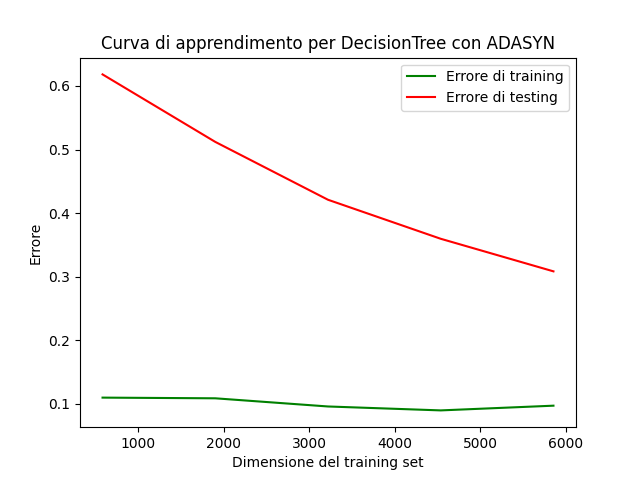
\includegraphics[scale=0.5]{img/learning_curve_DecisionTree_ADASYN.png}
      
    \end{minipage}
    \hfill
    \begin{minipage}[b]{0.45\linewidth}
      \centering
      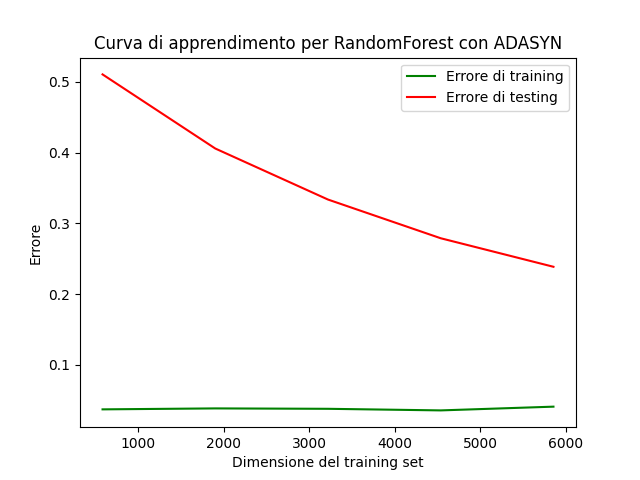
\includegraphics[scale=0.5]{img/learning_curve_RandomForest_ADASYN.png}
      
    \end{minipage}
    
    \begin{minipage}[b]{0.45\linewidth}
      \centering
      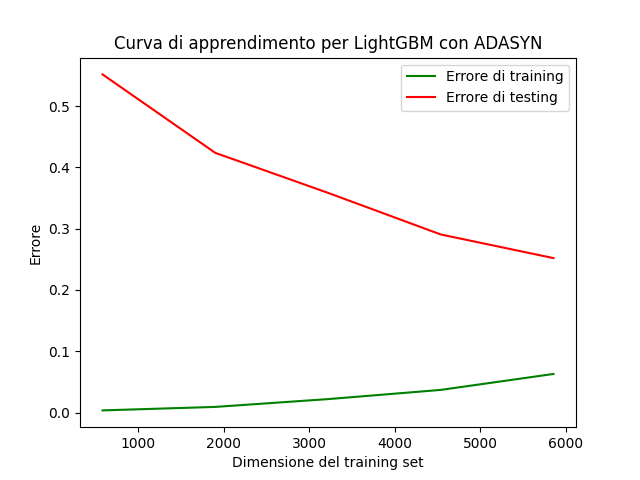
\includegraphics[scale=0.5]{img/learning_curve_LightGBM_ADASYN.png}
      
    \end{minipage}
    \hfill
    \begin{minipage}[b]{0.45\linewidth}
      \centering
      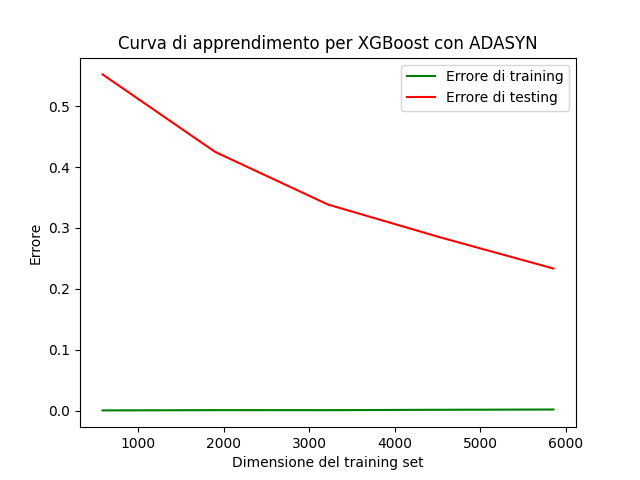
\includegraphics[scale=0.5]{img/learning_curve_XGBoost_ADASYN.png}
      
    \end{minipage}
    \caption{Curve di apprendimento.}
    
    \end{figure}

\begin{table}[H]
    \centering
    \begin{tabular}{lcc}
    \toprule
    \textbf{Modello} & \textbf{Train Error Std} & \textbf{Test Error Std} \\
    \midrule
    LightGBM & 0.0038361336791755867 & 0.014834571234512225 \\
    XGBoost & 0.0010135798069650331 & 0.01775432088891302 \\
    DecisionTree & 0.0050366494920735345 & 0.02674348515555034 \\
    RandomForest & 0.0028043557998990395 & 0.01884405548317221 \\
    \bottomrule
    \end{tabular}
    \caption{Deviazione standard dell'errore per i Modelli}
    
\end{table}

\begin{table}[H]
    \centering
    \begin{tabular}{lcc}
    \toprule
    \textbf{Modello} & \textbf{Train Error Var} & \textbf{Test Error Var} \\
    \midrule
    LightGBM & 1.4715921604505222e-05 & 0.00022006450371181758 \\
    XGBoost & 1.0273440250872736e-06 & 0.00031521591022649323 \\
    DecisionTree & 2.5367838106004596e-05 & 0.0007152139982651415\\
    RandomForest & 7.86441145242738e-06 & 0.00035509842705287254 \\
    \bottomrule
    \end{tabular}
    \caption{Varianza degli Errori per i Modelli}
    
\end{table}

\paragraph{Valutazione.} I punteggi sono simili agli esperimenti precedenti, ma non migliori dello SMOTE. \\ Random Forest e XGBoost risultano molto stabili, l'XGBoost sembra avere avere varianza e deviazione standard migliori, mentre LightGBM ancora una volta è in difficoltà. Il Decision Tree si comporta benino, ma risultando comunque il peggiore tra i modelli.


\subsection{Quarto esperimento: tecniche miste}
\noindent Non si è fatto uso di tecniche di undersampling, ovvero di tecniche che riducono il numero di esempi della classe maggioritaria, in quanto dopo un tentativo con un algoritmo di questo tipo (\textit{ClusterCentroids}, basato su \textit{K-Means}), i risultati erano imprensentabili, portando a scartare del tutto questa tecnica. In alternativa si proverà a utilizzare delle tecniche miste di oversampling e undersampling: SMOTEEEN e SMOTETomek, tecniche che applicano prima lo SMOTE per fare oversampling, per poi "pulire" il dataset, rimuovendo \textit{noise} e osservazioni "troppo facili da classificare", con tecniche di undersampling (EEN e Tomek).\\ Tomek rimuove quegli esempi di classi differenti che sono molto vicini tra loro, poichè saranno difficili da classificare e non aiutano l'algoritmo a trovare una discriminante. \\ EEN rimuove gli esempi di classe maggioritaria che sono molto vicini a quelli di classe minoritaria o gli esempi dove tutti o quasi i vicini sono di classi differenti, poichè potrebbero essere classificati erroneamente.

\subsubsection{SMOTETomek}
\paragraph{Iperparametri.} Di seguito si riportano gli iperparametri ottenuti dalla \textit{GridSearchCV} per ogni modello:

\begin{table}[H]
    \centering
    \begin{tabular}{|l|l|}
    \toprule
    \textbf{Parametro}                 & \textbf{Valore} \\ \midrule
    LightGBM\_\_learning\_rate            & 0.1             \\ 
    LightGBM\_\_max\_depth                & 10              \\ 
    LightGBM\_\_n\_estimators             & 200             \\ 
    LightGBM\_\_lambda                    & 0.01            \\ 
    LightGBM\_\_num\_leaves               & 15              \\ 
    LightGBM\_\_min\_gain\_to\_split      & 0.1             \\ 
    XGBoost\_\_learning\_rate         & 0.1             \\ 
    XGBoost\_\_max\_depth             & 10              \\ 
    XGBoost\_\_n\_estimators          & 100             \\ 
    XGBoost\_\_lambda                 & 0.01            \\ 
    DecisionTree\_\_criterion         & gini            \\ 
    DecisionTree\_\_max\_depth        & 20              \\ 
    DecisionTree\_\_min\_samples\_split & 2               \\ 
    DecisionTree\_\_min\_samples\_leaf & 2               \\ 
    RandomForest\_\_n\_estimators     & 200             \\ 
    RandomForest\_\_max\_depth        & 20              \\ 
    RandomForest\_\_min\_samples\_split & 2               \\ 
    RandomForest\_\_min\_samples\_leaf & 2               \\ 
    RandomForest\_\_criterion         & log\_loss       \\ \bottomrule
    \end{tabular}
    \caption{Parametri del modello}
    
    \end{table}

\paragraph{Risultati.} Di seguito si riportano i risultati ottenuti per ogni metrica e per ogni modello:
\begin{figure}[H]
    \centering
    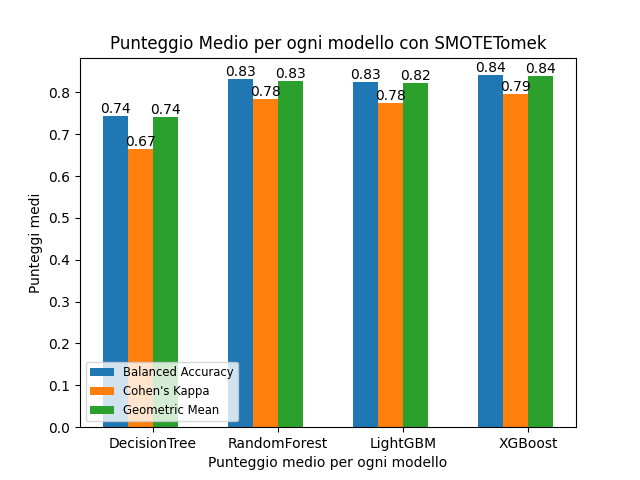
\includegraphics[scale=0.5]{img/tomek_metrics.png}
\end{figure}


\paragraph{Curve di apprendimento.} Di seguito si riportano le curve di apprendimento per ogni modello, con tanto di deviazione standard e varianza:

\begin{figure}[H]
    \centering
    \begin{minipage}[b]{0.45\linewidth}
      \centering
      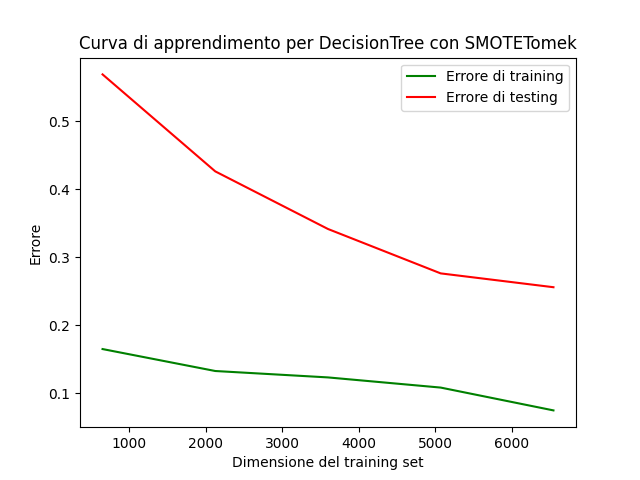
\includegraphics[scale=0.5]{img/learning_curve_DecisionTree_SMOTETomek.png}
      
    \end{minipage}
    \hfill
    \begin{minipage}[b]{0.45\linewidth}
      \centering
      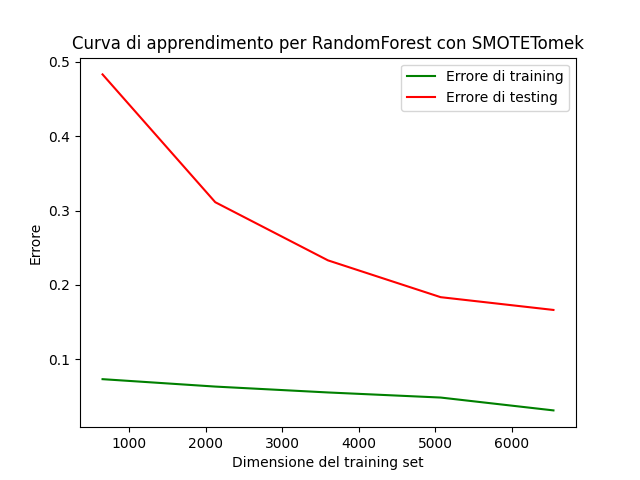
\includegraphics[scale=0.5]{img/learning_curve_RandomForest_SMOTETomek.png}
      
    \end{minipage}
    
    \begin{minipage}[b]{0.45\linewidth}
      \centering
      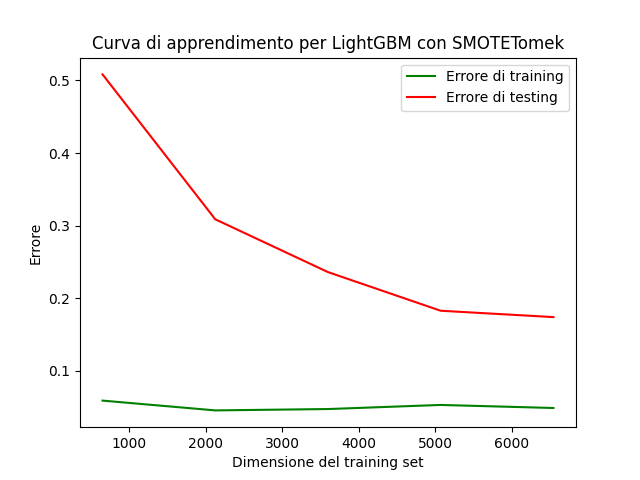
\includegraphics[scale=0.5]{img/learning_curve_LightGBM_SMOTETomek.png}
      
    \end{minipage}
    \hfill
    \begin{minipage}[b]{0.45\linewidth}
      \centering
      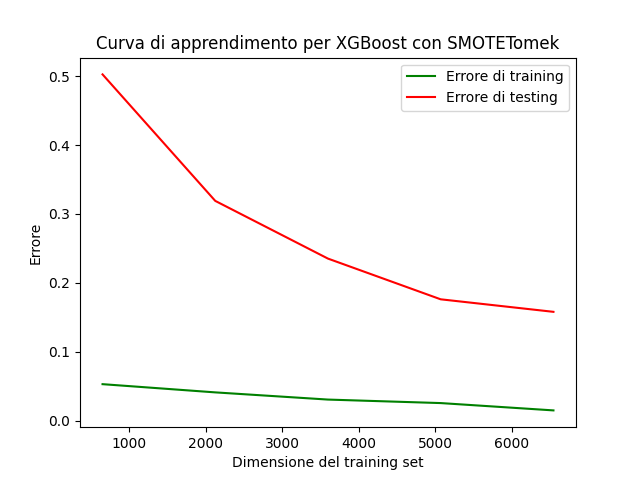
\includegraphics[scale=0.5]{img/learning_curve_XGBoost_SMOTETomek.png}
      
    \end{minipage}
    \caption{Curve di apprendimento.}
    
    \end{figure}

\begin{table}[H]
    \centering
    \begin{tabular}{lcc}
    \toprule
    \textbf{Modello} & \textbf{Train Error Std} & \textbf{Test Error Std} \\
    \midrule
    LightGBM & 0.0023555215150484524 & 0.009308465169567823 \\
    XGBoost & 0.0007603005596334415 & 0.007147550348338646 \\
    DecisionTree & 0.004106118784835311 & 0.010978248717168952 \\
    RandomForest & 0.001156335935796055 & 0.005023366391826634 \\
    \bottomrule
    \end{tabular}
    \caption{Deviazione standard dell'errore per i Modelli}
    
\end{table}

\begin{table}[H]
    \centering
    \begin{tabular}{lcc}
    \toprule
    \textbf{Modello} & \textbf{Train Error Var} & \textbf{Test Error Var} \\
    \midrule
    LightGBM & 5.548481607856157e-06 & 8.664752381305731e-05 \\
    XGBoost & 5.780569409789242e-07 & 5.1087475982035904e-05 \\
    DecisionTree & 1.6860211475177415e-05 & 0.00012052194489602173 \\
    RandomForest & 1.3371127964133382e-06 & 2.523420990653334e-05 \\
    \bottomrule
    \end{tabular}
    \caption{Varianza degli Errori per i Modelli}
    
\end{table}

\paragraph{Valutazione.} I risultati sono simili all'esperimento con SMOTE. \\ Varianza e deviazione standard sono nella maggior parte dei casi maggiori rispetto all'esperimento con SMOTE e in generale i modelli sembrano aver bisogno di più dati per apprendere, notiamo come l'errore di training non si stabilizza in nessuno dei modelli.

\subsubsection{SMOTEENN}
\paragraph{Iperparametri.} Di seguito si riportano gli iperparametri ottenuti dalla \textit{GridSearchCV} per ogni modello:

\begin{table}[H]
    \centering
    \begin{tabular}{|l|l|}
    \toprule
    \textbf{Parametro}                 & \textbf{Valore} \\ \midrule
    LightGBM\_\_learning\_rate            & 0.05            \\ 
    LightGBM\_\_max\_depth                & 5               \\ 
    LightGBM\_\_n\_estimators             & 200             \\ 
    LightGBM\_\_lambda                    & 0.1             \\ 
    LightGBM\_\_num\_leaves               & 15              \\ 
    LightGBM\_\_min\_gain\_to\_split      & 0.1             \\ 
    XGBoost\_\_learning\_rate         & 0.1             \\ 
    XGBoost\_\_max\_depth             & 20              \\ 
    XGBoost\_\_n\_estimators          & 100             \\ 
    XGBoost\_\_lambda                 & 0.1             \\ 
    DecisionTree\_\_criterion         & log\_loss       \\ 
    DecisionTree\_\_max\_depth        & 40              \\ 
    DecisionTree\_\_min\_samples\_split & 2               \\ 
    DecisionTree\_\_min\_samples\_leaf & 2               \\ 
    RandomForest\_\_n\_estimators     & 100             \\ 
    RandomForest\_\_max\_depth        & 20              \\ 
    RandomForest\_\_min\_samples\_split & 2               \\ 
    RandomForest\_\_min\_samples\_leaf & 2               \\ 
    RandomForest\_\_criterion         & gini            \\ \bottomrule
    \end{tabular}
    \caption{Parametri del modello}
    
    \end{table}

\paragraph{Risultati.} Di seguito si riportano i risultati ottenuti per ogni metrica e per ogni modello:

\begin{figure}[H]
    \centering
    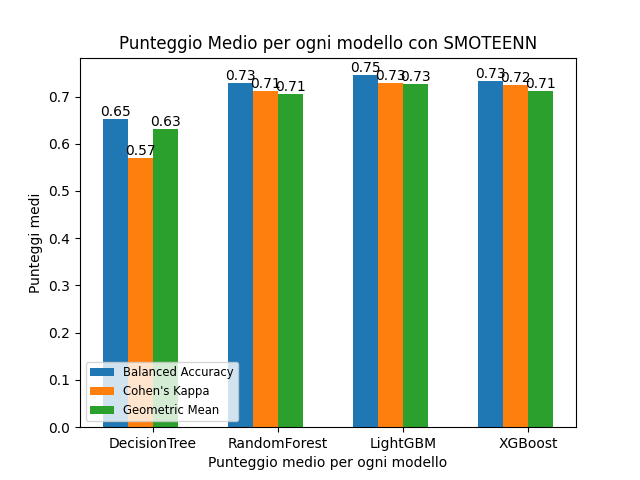
\includegraphics[scale=0.7]{img/smoteen_metrics.png}
\end{figure}



\paragraph{Curve di apprendimento.} Di seguito si riportano le curve di apprendimento per ogni modello, con tanto di deviazione standard e varianza:

\begin{figure}[H]
    \centering
    \begin{minipage}[b]{0.45\linewidth}
      \centering
      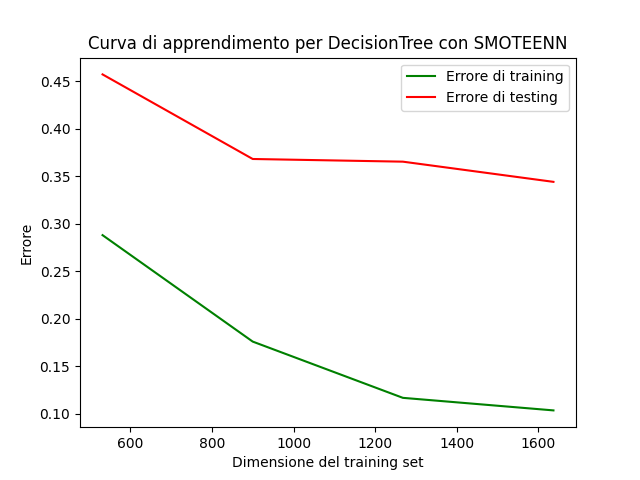
\includegraphics[scale=0.5]{img/learning_curve_DecisionTree_SMOTEENN.png}
      
    \end{minipage}
    \hfill
    \begin{minipage}[b]{0.45\linewidth}
      \centering
      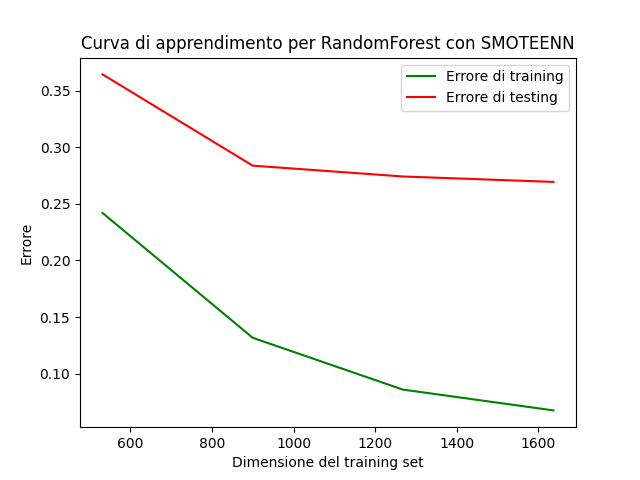
\includegraphics[scale=0.5]{img/learning_curve_RandomForest_SMOTEENN.png}
      
    \end{minipage}
    
    \begin{minipage}[b]{0.45\linewidth}
      \centering
      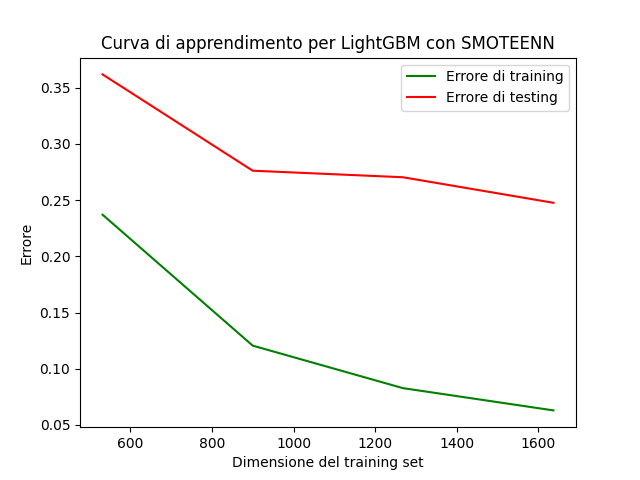
\includegraphics[scale=0.5]{img/learning_curve_LightGBM_SMOTEENN.png}
      
    \end{minipage}
    \hfill
    \begin{minipage}[b]{0.45\linewidth}
      \centering
      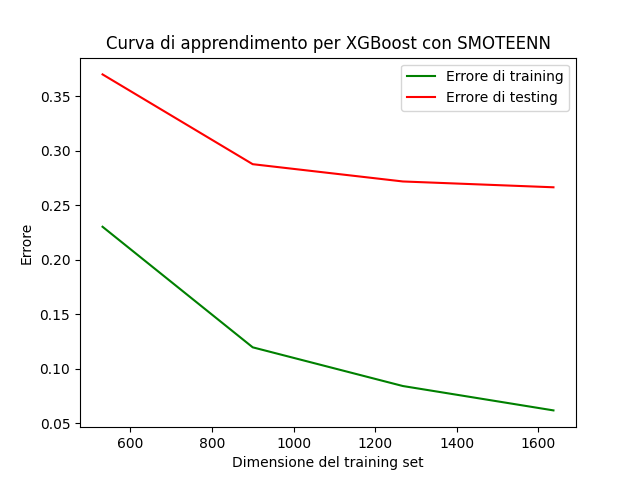
\includegraphics[scale=0.5]{img/learning_curve_XGBoost_SMOTEENN.png}
      
    \end{minipage}
    \caption{Curve di apprendimento.}
    
    \end{figure}


\begin{table}[H]
    \centering
    \begin{tabular}{lcc}
    \toprule
    \textbf{Modello} & \textbf{Train Error Std} & \textbf{Test Error Std} \\
    \midrule
    LightGBM & 0.00686144408303901 & 0.02657900599318599 \\
    XGBoost & 0.007076483753736052 & 0.025883027531329383 \\
    DecisionTree & 0.00943035445191201 & 0.020224378283450403 \\
    RandomForest & 0.00802437542204398 & 0.03194225646631045 \\
    \bottomrule
    \end{tabular}
    \caption{Deviazione standard dell'errore per i Modelli}
    
\end{table}

\begin{table}[H]
    \centering
    \begin{tabular}{lcc}
    \toprule
    \textbf{Modello} & \textbf{Train Error Var} & \textbf{Test Error Var} \\
    \midrule
    LightGBM & 4.707941490467104e-05 & 0.0007064435595858169 \\
    XGBoost & 5.007662231689027e-05 & 0.0006699311141875547\\
    DecisionTree & 8.893158508869667e-05 & 0.00040902547695210025 \\
    RandomForest & 6.439060091390349e-05 & 0.0010203077481595517\\
    \bottomrule
    \end{tabular}
    \caption{Varianza degli Errori per i Modelli}
    
\end{table}

\paragraph{Valutazione.} I risultati sono al pari dei primi esperimenti, se non inferiori. \\ Dalle curve di apprendimento si può facilmente notare come i modelli non siano riusciti a stabilizzarsi, e la varianza e la deviazione standard sono molto alte, segno che i modelli non sono riusciti a generalizzare bene. Il numero di esempi non era sufficiente.

\subsection{Sommario}
\noindent In generale, i risultati avuti sono accettabili. Non vi è un modello che spicca rispetto a tutti, ma ciò che possiamo affermare con certezza è che l'esperimento con SMOTE è quello globalmente andato meglio. I modelli che si sono distinti sono stati: 
\begin{itemize}[label=-]
    \item l'XGBoost del primo esperimento, simile per risultati, deviazione standard e varianza al Random Forest del primo esperimento ma con una curva di apprendimento migliore;
    \item il Random Forest del secondo esperimento;
    \item il Random Forest e l'XGBoost del terzo esperimento con SMOTE, risultati i migliori globalmente;
    \item l'XGBoost del terzo esperimento con ADASYN;
    \item l'XGBoost del quarto esperimento con SMOTETomek.
\end{itemize}

\noindent Un possibile approccio futuro può essere quello di combinare i modelli che si sono distinti per verificare se i risultati sono migliorabili.
